The requeriments of the water purification system are:

\begin{enumerate}

\item{} A high degree of purification of the water sample extracted from the dam, reducing its conductivity by approximately two orders of magnitude (from $1000~\mu$S$/\cm$ to $10~\mu$S$/\cm$).

\item{} Low maintenance cost  and manpower.

\item{} Remote management of the system.
\end{enumerate}

The LARUEX laboratory designed and built the water purification system, which scheme is shown in Figure \ref{fig:WPSScheme}.

\begin{figure}[htbp]
\centering
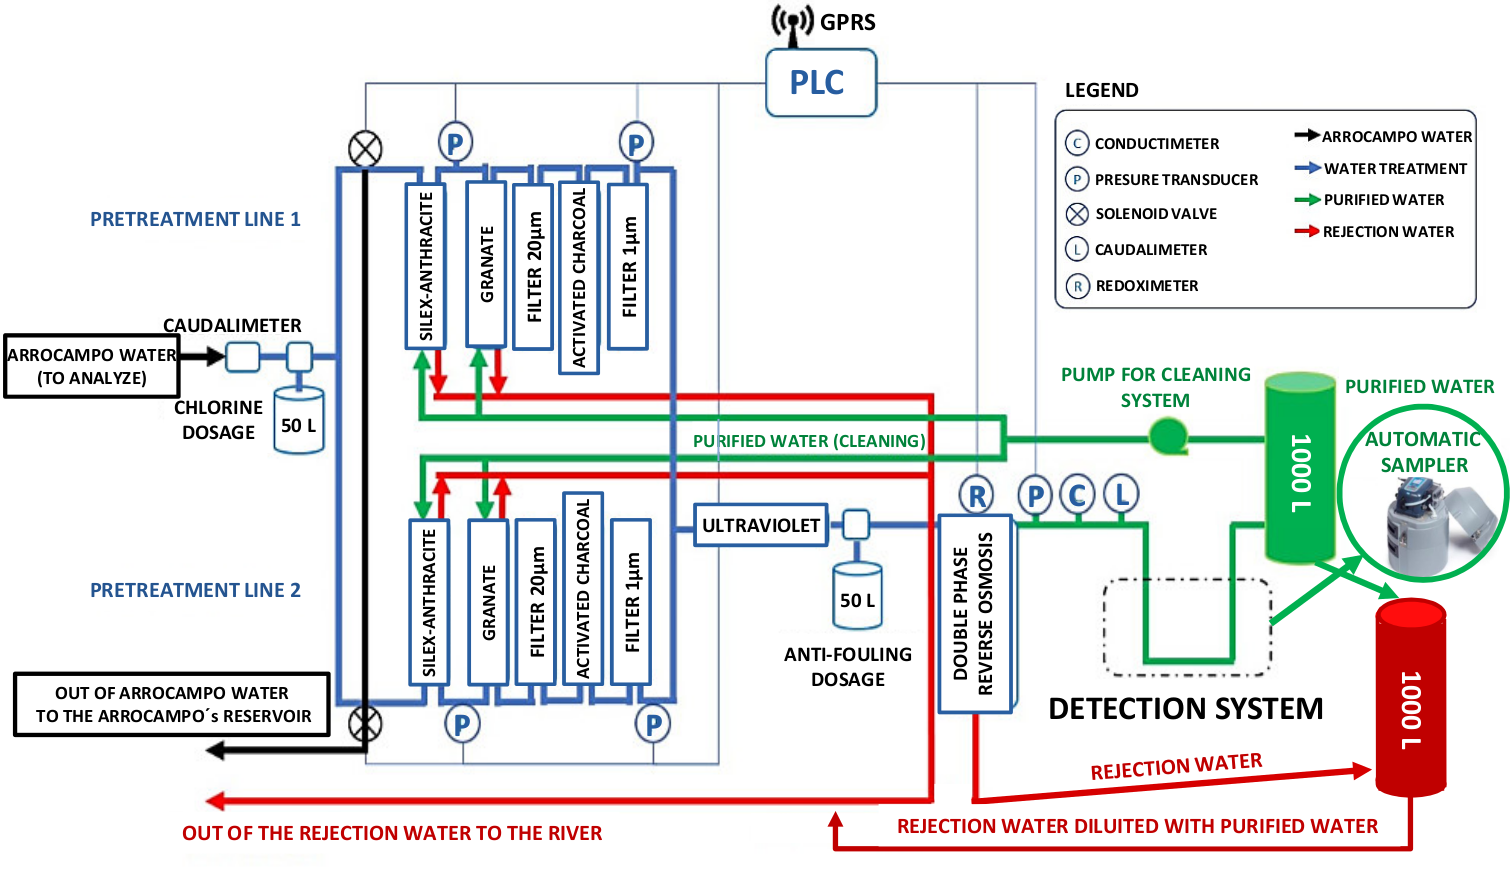
\includegraphics[scale=0.25]{3DesignPrinciples/33UltraPureWaterSystem/SchemeUltraPureWaterSystem.png}
\caption{Scheme of the water purification system of TRITIUM.\label{fig:WPSScheme}}
\end{figure}
This system is installed in the Arrocampo site and consists of four different stages:

\begin{enumerate}
\item{} The raw water from the Tagus river passes through two different filters, the first made of silex-anthracite and the second of garnet, with which a rough filtering is made (the largest particles are eliminated). This system has two identical parallel lines and implements a self-cleaning function by injecting purified water in the opposite direction.

\item{} The outlet water from the first stage, called fine filtration stage, passes through a $20~\mu\meter$ filter (formed by a synthetic mesh) and activated charcoal filters (one per line) that remove chlorine and iron particles present in the water.

\item{} The outlet water from the second stage goes into a super-fine filtering stage consisting of a $1~\mu\meter$ filter, made of a dense polypropylene mesh and of UV lamps. The filter removes all the particles with a diameter larger than $1~\mu\meter$ and the UV lamps sterilize the water, eliminating bacteria and microscopic life.

\item{} Finally, the water is introduced into the last stage that consists of a double-phase reverse osmosis which  reduces the conductivity of the water to about $10~\mu\mathrm{S}/\cm$. 

\end{enumerate}

As a result of the purification process, besides the pure water that is introduced into the TRITIUM detector, a rejection water is produced,  which contains the particles removed from the sample. The water purification system is able to process up to $0.850~\meter^3/\hour$ with a single operating line or $1.480~\meter^3/\hour$ with both lines.

The software used for remote controlling the water purification system is the Siemens Programmable Logic Controller (Siemens PLC), that gives information such as the state of the valves, the reading of pressure probes and the amount of ultrapure water production in real time. The appendix \ref{App:UltraPureWaterSystem} contains several pictures of different parts of this system.